%! Author = chtompki
%! Date = 1/14/26
\documentclass[12pt]{amsart}
% Default margins are too wide all the way around. I reset them here
\setlength{\hoffset}{-.75in}
\setlength{\textwidth}{6.5in}
\setlength{\voffset}{-.5in}
\setlength{\textheight}{9.0in}
\usepackage{amsmath}
\usepackage{amssymb}
\usepackage{amsthm}
\usepackage{enumitem}
\usepackage{setspace}
\usepackage{graphicx}
\usepackage{listings}
\usepackage{pgfplots}
\usepackage{booktabs}
\usepackage{xcolor}
\usepackage[colorlinks=true, urlcolor=black, linkcolor=black]{hyperref}

\newenvironment{solution}
{\begin{proof}[Solution]}
{\end{proof}}

\newcommand{\dd}{\mathop{}\!\mathrm{d}}

\title{Numerical Analysis\\Guided Lab 4}
\author{Rob Tompkins}
\date{\today}

\begin{document}
    \maketitle
    \date{\today}
    \begin{onehalfspace}
        Note, all the files associated with Guided Lab 4 are checked into the : \\
        \underline{https://github.com/chtompki/MathSpring2026/tree/main/NumericalAnalysis/GuidedLab4}\\
\quad\\

        \noindent\textbf{1.} Given an intial value problem $y'=f(t,y)$ for $t\in[a,b]$ with initial condition $y(a)=\alpha$,
        create a program that implements RK4 to approximate the solution $w_i\approx y(t_i)$ with
        fixed step-size $h=(b-a)/N$:
        \begin{align*}
            k_1 &= h f(t_i,w_i)\\
            k_2 &= h f\left(t_i+\frac h2,w_i+\frac{k_1}{2}\right)\\
            k_3 &= h f\left(t_i+\frac h2,w_i+\frac{k_2}{2}\right)\\
            k_4 &= h f(t_i+h,w_i+k_3)\\
            w_{i+1} &= w_i+\frac16(k_1+2k_2+2k_3+k_4)
        \end{align*}
        \vspace{7pt}
        Be sure to design your code to be able to handle systems of equations (e.g. $y\in\mathbb R^n$).
        You may find the Matlab tutorial found at \href{https://ocw.mit.edu/courses/res-18-009-learn-differential-equations-up-close-with-gilbert-strang-and-cleve-moler-fall-2015/resources/classical-runge-kutta-ode4/}{this link} helpful.

        \begin{solution}
            The classical fourth-order Runge--Kutta method can be implemented directly
            from the formulas above. To allow the same routine to handle both a scalar
            differential equation and a system of differential equations, the numerical
            solution is treated internally as a column vector. Thus, if
            \[
                y(t)=
                \begin{bmatrix}
                    y_1(t)\\
                    \vdots\\
                    y_n(t)
                \end{bmatrix},
            \]
            then \(f(t,y)\) returns an \(n\times1\) column vector.

            For a fixed number of steps \(N\), define
            \[
                h=\frac{b-a}{N}
            \]
            and
            \[
                t_i=a+ih,\qquad i=0,1,\ldots,N.
            \]
            Starting with
            \[
                w_0=\alpha,
            \]
            the RK4 approximation is computed for \(i=0,\ldots,N-1\) using
            \begin{align*}
                k_1 &= h f(t_i,w_i),\\
                k_2 &= h f\left(t_i+\frac{h}{2},
                w_i+\frac{k_1}{2}\right),\\
                k_3 &= h f\left(t_i+\frac{h}{2},
                w_i+\frac{k_2}{2}\right),\\
                k_4 &= h f(t_i+h,w_i+k_3),
            \end{align*}
            followed by
            \[
                w_{i+1}
                =
                w_i+\frac{1}{6}\left(k_1+2k_2+2k_3+k_4\right).
            \]

            The following Matlab function implements this algorithm.

            \begin{lstlisting}
                function [t,w] = rk4(f,a,b,alpha,N)
                %RK4 Classical fourth-order Runge-Kutta method.
                %
                % [t,w] = rk4(f,a,b,alpha,N)
                %
                % Approximates the solution of
                %
                %     y' = f(t,y),    a <= t <= b,
                %     y(a) = alpha,
                %
                % using N equally spaced RK4 steps.

                    h = (b-a)/N;

                    % Convert the initial condition to a column vector.
                    alpha = alpha(:);
                    n = length(alpha);

                    % Construct the time mesh.
                    t = linspace(a,b,N+1).';

                    % Preallocate storage for the numerical solution.
                    % Each row contains one approximation.
                    w = zeros(N+1,n);
                    w(1,:) = alpha.';

                    for i = 1:N

                        % Current approximation as a column vector.
                        wi = w(i,:).';

                        k1 = h*f(t(i),wi);

                        k2 = h*f(t(i) + h/2, ...
                                 wi + k1/2);

                        k3 = h*f(t(i) + h/2, ...
                                 wi + k2/2);

                        k4 = h*f(t(i) + h, ...
                                 wi + k3);

                        wi_next = wi + ...
                            (k1 + 2*k2 + 2*k3 + k4)/6;

                        w(i+1,:) = wi_next.';
                    end
                end
            \end{lstlisting}

            For example, for the scalar initial value problem
            \[
                y'=y-t^2+1,\qquad y(0)=0.5,
            \]
            on \(0\leq t\leq2\), the routine can be called using
            \begin{lstlisting}
                f = @(t,y) y - t.^2 + 1;

                [t,w] = rk4(f,0,2,0.5,10);

                disp([t,w])

                %========Outputs======
                % >> gl4prob1
                % 0    0.5000
                % 0.2000    0.8293
                % 0.4000    1.2141
                % 0.6000    1.6489
                % 0.8000    2.1272
                % 1.0000    2.6408
                % 1.2000    3.1799
                % 1.4000    3.7323
                % 1.6000    4.2834
                % 1.8000    4.8151
                % 2.0000    5.3054
            \end{lstlisting}

            The same routine works without modification for a system. For example,
            consider
            \[
                \begin{aligned}
                    y_1' &= y_2,\\
                    y_2' &= -y_1,
                \end{aligned}
                \qquad
                y_1(0)=0,\qquad y_2(0)=1.
            \]
            Writing the system in vector form gives
            \[
                y'=
                \begin{bmatrix}
                    y_2\\
                    -y_1
                \end{bmatrix}.
            \]
            The corresponding Matlab code is
            \begin{lstlisting}
                f = @(t,y) [y(2); -y(1)];

                alpha = [0;1];

                [t,w] = rk4(f,0,2*pi,alpha,100);

                plot(t,w(:,1),'LineWidth',1.5)
                hold on
                plot(t,w(:,2),'LineWidth',1.5)
                legend('y_1','y_2')
                xlabel('t')
                ylabel('Approximate solution')
                grid on
            \end{lstlisting}

            This code yields the plot in Figure \ref{gl1prob1fig1} below:

            \begin{figure}[!ht]
                \centering
                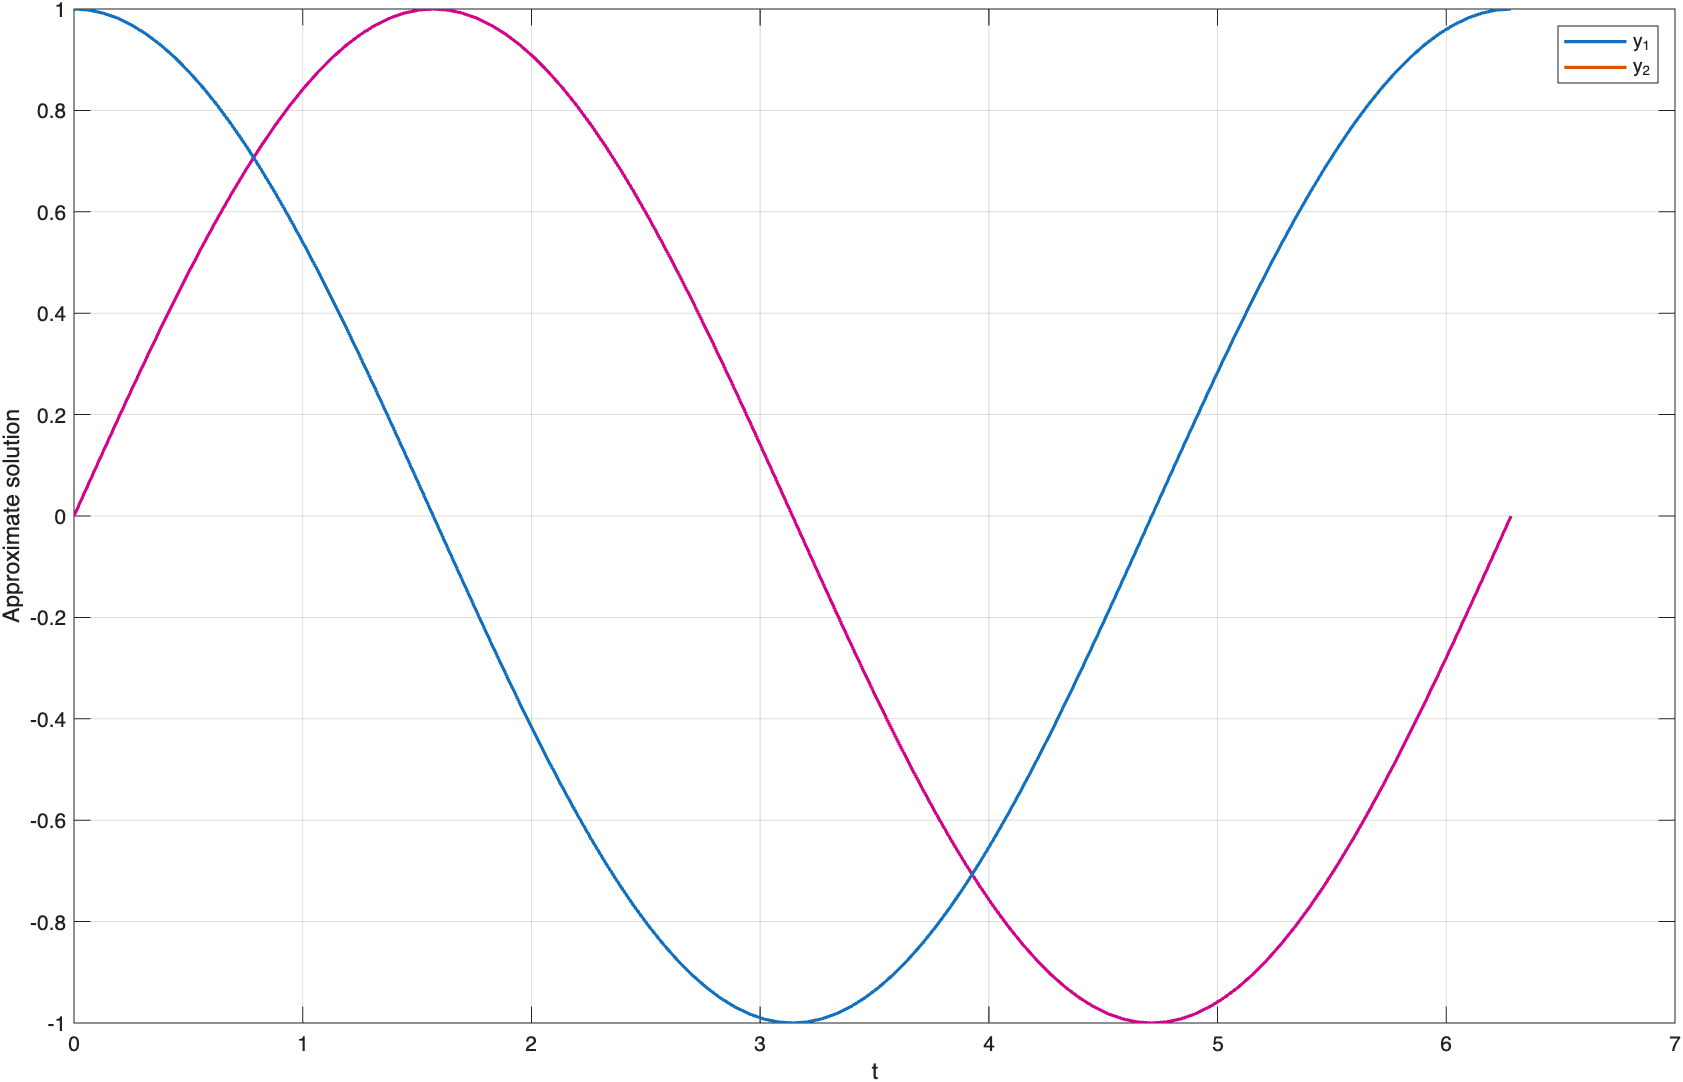
\includegraphics[scale=0.5]{Prob1Figure1.png}
                \caption{A solution for $y'_1 = y_2$ and $y'_2 = -y_1$.}
                \label{gl1prob1fig1}.
            \end{figure}

            Because \(w_i\), \(k_1\), \(k_2\), \(k_3\), and \(k_4\) may all be vectors,
            the RK4 formulas are unchanged when solving a system of equations. The
            classical RK4 method has global truncation error
            \[
                O(h^4).
            \]
            Consequently, in the asymptotic error regime, reducing the step size by a
            factor of two reduces the global discretization error by approximately
            \(2^4=16\).
        \end{solution}

        \newpage
        \noindent\textbf{2.} Consider the initial value problem
        \begin{equation}
            \frac{\dd y}{\dd t}=1-y+e^{2t}y^2\quad(0\le t\le0.9),\qquad y(0)=0
        \end{equation}
        \begin{enumerate}
            \item Verify that the exact solution is $y(t)=e^{-t}\tan(e^t-1)$.
            \item Use your RK4 code to approximate the solution to the given initial value problem,
            using a stepsize of $h=0.1$. Store the approximate solution at each time step as
            an element in a vector $w$. Also add a vector to your code which stores the errors,
            $err=x-w$.

            \item Set up a script that solves the initial value problem for different step sizes $10^{-9}\le
            h\le10^{-1}$ and stores the error at $t=0.9$. Run this script on VCU's Athena cluster
            by submitting it as batch job (not interactively!). More information on how to do
            this can be found \href{https://wiki-vcu.atlassian.net/wiki/spaces/unix/pages/45973545/Athena+cluster}{here}). If you are using Matlab, you can find an example script
            for submitting your job \href{https://wiki-vcu.atlassian.net/wiki/spaces/unix/pages/45975823/Module+Matlab}{here}. Make a log-log plot of the error vs. the stepsize
            and use this to verify the method converges with rate $O(h^4)$.

            \vspace{2pt}
            \underline{challenge:} Assuming your code stores the solution at every step, you will likely
            become memory-limited if you try to test convergence using smaller step sizes.
            Modify your code to only save the final value of the solution, and go down to step
            sizes small enough to observe the effects of round-off error.
        \end{enumerate}

        \begin{solution}
            Note athena output files can be found at \underline{https://github.com/chtompki/MathSpring2026/tree/main/NumericalAnalysis/GuidedLab4/athena-files}
            \section*{1. Verification of the exact solution}
            Let $u=e^t-1$ and $y=e^{-t}\tan u$. Differentiating gives
            \begin{align*}
                y'&=-e^{-t}\tan u+e^{-t}\sec^2u\,e^t\\
                &=-y+1+\tan^2u=1-y+e^{2t}y^2.
            \end{align*}
            Also $y(0)=\tan 0=0$, so
            \[
                \boxed{y(t)=e^{-t}\tan(e^t-1).}
            \]
            The first positive pole occurs at $t_* = \log(1+\pi/2)\approx0.944216$,
            which lies beyond $0.9$. Thus the solution is smooth throughout the
            requested interval. Since $f(t,y)=1-y+e^{2t}y^2$ is locally Lipschitz in
            $y$, this is the unique solution there.

            \section*{2. Classical RK4 with $h=0.1$}
            Set $t_n=nh$, $w_0=0$, and compute
            \begin{align*}
                k_1&=f(t_n,w_n), & k_2&=f(t_n+h/2,w_n+hk_1/2),\\
                k_3&=f(t_n+h/2,w_n+hk_2/2), & k_4&=f(t_n+h,w_n+hk_3),\\
                w_{n+1}&=w_n+\frac{h}{6}(k_1+2k_2+2k_3+k_4).
            \end{align*}
            In MATLAB, entry $n+1$ represents time $t_n$; the vectors include the
            initial value. The code sets \texttt{x=exp(-t).*tan(expm1(t))} and
            \texttt{err=x-w}, preserving the requested signed errors.
            \begin{center}\small
                \begin{tabular}{rrrr}\toprule
                    $t_n$ & $x_n=y(t_n)$ & $w_n$ & $x_n-w_n$\\\midrule
                    0.0 & 0.0000000000 & 0.0000000000 & 0.00000e+00 \\
                    0.1 & 0.0955150033 & 0.0955152528 & -2.49549e-07 \\
                    0.2 & 0.1842903884 & 0.1842907307 & -3.42349e-07 \\
                    0.3 & 0.2703012310 & 0.2703013801 & -1.49077e-07 \\
                    0.4 & 0.3591134152 & 0.3591129732 & 4.42060e-07 \\
                    0.5 & 0.4598646541 & 0.4598633897 & 1.26439e-06 \\
                    0.6 & 0.5906730569 & 0.5906721448 & 9.12094e-07 \\
                    0.7 & 0.7972935784 & 0.7972918936 & 1.68477e-06 \\
                    0.8 & 1.2493126185 & 1.2487983913 & 5.14227e-04 \\
                    0.9 & 3.6413433579 & 3.4902224437 & 1.51121e-01 \\
                    \bottomrule\end{tabular}
            \end{center}
            In particular, $y(0.9)\approx3.64134335794140$ and
            $w_9\approx3.49022244367240$, with signed error
            $0.15112091426900$. The relatively large error at this coarse step size
            reflects the rapid growth near the pole.

            \newpage
            \section*{3. Convergence experiment and interpretation}
            The supplied script \texttt{rk4\_ivp\_solution.m} uses
            \[
                h_j=10^{-j},\quad N_j=9\cdot10^{j-1},\quad j=1,\ldots,9,
                \qquad E(h)=|y(0.9)-w_N|.
            \]
            Internally it sets $h=0.9/N$ and computes time from $t_n=nh$, avoiding
            repeated floating-point addition of the time variable. Successive
            observed orders are
            \[
                p_j=\frac{\log(E(h_{j-1})/E(h_j))}{\log(h_{j-1}/h_j)}.
            \]
            \textbf{Verification status.} The following table and plot were computed
            locally with an independent Python implementation of the same RK4
            formulas in double precision. MATLAB and an authenticated Athena session
            were not available for this preparation. These are not Athena job results.
            The supplied MATLAB program performs the full requested sweep through
            $10^{-9}$ and writes its own tables, timing data, and plot.
            \begin{center}
                \begin{tabular}{rrrr}\toprule
                    $h$ & Steps $N$ & $E(h)$ & Observed order\\\midrule
                    $10^{-1}$ & 9 & 1.511209e-01 & -- \\
                    $10^{-2}$ & 90 & 7.370413e-05 & 3.3118 \\
                    $10^{-3}$ & 900 & 7.161237e-09 & 4.0125 \\
                    $10^{-4}$ & 9,000 & 7.100986e-13 & 4.0037 \\
                    $10^{-5}$ & 90,000 & 2.087219e-14 & 1.5318 \\
                    $10^{-6}$ & 900,000 & 8.397727e-13 & -1.6046 \\
                    \bottomrule\end{tabular}
            \end{center}
            \begin{center}
                \begin{tikzpicture}
                    \begin{loglogaxis}[width=0.92\linewidth,height=6.4cm,
                    xlabel={Step size $h$},ylabel={Absolute endpoint error $E(h)$},
                    grid=both,legend pos=north west,legend style={font=\small},
                    xmin=5e-7,xmax=0.2,ymin=1e-21,ymax=1,
                    log basis x=10,log basis y=10]
                        \addplot+[mark=*,thick] coordinates {(0.1,0.151120914269) (0.01,7.37041332965e-05) (0.001,7.16123693678e-09) (0.0001,7.1009864655e-13) (1e-05,2.0872192863e-14) (1e-06,8.39772695826e-13)};
                        \addlegendentry{Local independent verification}
                        \addplot[black,dashed,domain=1e-6:1e-1,samples=2] {7161.23693678*x^4};
                        \addlegendentry{$C h^4$ reference}
                    \end{loglogaxis}
                \end{tikzpicture}
            \end{center}
            The orders $4.0125$ and $4.0037$ confirm fourth-order behavior in the
            truncation-dominated range. RK4 has one-step defect $O(h^5)$, which gives
            global error $O(h^4)$ on this fixed smooth interval. The coarse step
            $h=0.1$ is not yet in that asymptotic range. A slope fitted over the entire
            range, including round-off-dominated points, would not estimate the
            method's order reliably.

            \newpage
            \section*{4. Challenge: constant memory and round-off}
            Storing one double-precision vector at $h=10^{-9}$ requires approximately
            \[
                8(N+1)=8(900{,}000{,}001)\ \text{bytes}\approx7.2\ \text{GB}.
            \]
            Four full vectors ($t,x,w,err$) require about $28.8$ GB before temporary
            arrays and MATLAB overhead. The convergence solver instead keeps only
            the current scalar $y$, the scalar time and index, and four RK stages.
            Its working storage is $O(1)$ in the number of steps. It uses a scalar
            \texttt{while} loop and never constructs a full grid for the fine runs.
            The ten-entry vectors required in part 2 are still retained.

            Constant memory does not remove the computational cost: the finest run
            requires $9\times10^8$ steps, and all nine runs require $999{,}999{,}999$
            steps. Runtime remains $O(1/h)$. Results are saved after each completed
            step size so that a batch time limit does not erase earlier runs.

            In exact arithmetic, the discretization error continues decreasing like
            $h^4$. In floating-point arithmetic, rounding in stage evaluations and
            updates eventually dominates. Already in the local check, the error
            falls to approximately $2.1\times10^{-14}$ at $h=10^{-5}$ and rises to
            approximately $8.4\times10^{-13}$ at $h=10^{-6}$. The detailed values
            and turning point depend on the platform and arithmetic evaluation.
            The double-precision evaluation of the exact endpoint also limits the
            accuracy of the reported error near machine precision.

            A useful qualitative model is
            \[
                E(h)\lesssim C_T h^4+C_R\frac{u}{h},
            \]
            where $u$ denotes unit round-off. The second term is a pessimistic
            accumulation model, not a universal measured law; less correlated
            round-off can grow more slowly. Perturbations can also be amplified by
            $f_y=-1+2e^{2t}y$ along this rapidly growing solution. The expected plot
            therefore decreases with slope approximately four before flattening or
            becoming irregular and increasing. Zero computed errors, if any, are
            omitted from the log-log plot and reported by the script.

            \section*{5. Running the supplied files}
            For a short MATLAB check (down to $10^{-5}$), run:
            \begin{lstlisting}
setenv('RK4_QUICK','1');
rk4_ivp_solution
            \end{lstlisting}
            The full experiment is enabled by default. Submit it on Athena as a
            batch job using the included \texttt{athena\_rk4.slurm}; do not execute
            the full experiment on a login node.

            \section*{6. Athena batch submission}
            Place \texttt{rk4\_ivp\_solution.m} and \texttt{athena\_rk4.slurm}
            in the same writable directory on Athena. From that directory submit:
            \begin{lstlisting}[language=bash]
sbatch athena_rk4.slurm
squeue -u "$USER"
            \end{lstlisting}
            The batch file is:
            \begin{lstlisting}[language=bash]
#!/bin/bash
#SBATCH --job-name=rk4_ivp
#SBATCH --output=rk4_%j.out
#SBATCH --error=rk4_%j.err
#SBATCH --cpus-per-task=1
#SBATCH --mem=4G
#SBATCH --time=1-00:00:00

set -e
cd "$SLURM_SUBMIT_DIR"
module load matlab/R2024a
export RK4_QUICK=0
matlab -singleCompThread -batch "rk4_ivp_solution"
            \end{lstlisting}
            The one-day wall-time request is a starting allowance, not a runtime
            prediction; adjust it to the applicable queue limits and measured speed.
            Only one CPU is requested because each trajectory is advanced serially.
            The module and submission command follow VCU's
            \href{https://wiki-vcu.atlassian.net/wiki/spaces/unix/pages/45975823}{MATLAB module instructions};
            also see the
            \href{https://wiki-vcu.atlassian.net/wiki/spaces/unix/pages/45973545}{Athena cluster guide}
            (documentation checked September 15, 2026).

            The program writes \texttt{rk4\_nodes.csv/.mat},
            \texttt{rk4\_convergence.csv/.mat}, and
            \texttt{rk4\_convergence.pdf/.png} alongside the MATLAB script.
            The convergence CSV contains the step size, step count, final value,
            signed and absolute errors, observed order, and elapsed seconds.
            Do not launch overlapping runs into the same output directory.

            To finish the cluster-specific part of the assignment, retain the job ID
            and logs, verify that all nine rows through $h=10^{-9}$ are present, and
            use the generated MATLAB plot in the submitted report. No cluster job
            submission or completion is claimed in this document.
        \end{solution}

        \noindent\textbf{3.} You will now use your RK4 code to reproduce figure 7.21 in your textbook. Consider
        the model for cell production in a chemostat
        \begin{align*}
            \dot{s}&=1-s-\frac{msx}{a+s}\\
            \dot{x}&=\frac{msx}{a+s}-x
        \end{align*}
        with $m=16$ and $a=0.25$.
        \begin{enumerate}
            \item Find the fixed points of the system and determine their stability.
            \item Apply RK4 with step size $h=0.05$ to approximate the solution to the initial value
            problem for $0\le t\le12$ with intial conditions $s(0)=0.5$ and $x(0)=0.02$. Plot
            $s(t)$ and $x(t)$ and explain how your results are consistent to your linear stability
            analysis.
            \item Now repeat the previous part, this time using $h=0.06$ to approximate the
            solution. Comment on the differences in your plots for $s(t)$ and $x(t)$.
        \end{enumerate}

        \begin{solution}
            \leavevmode\par
            \subsection*{1. Fixed points and their stability}
            Adding the two equations gives
            \[
                (s+x)'=1-(s+x).
            \]
            Consequently every fixed point satisfies $s+x=1$. The second equation
            also requires
            \[
                x\left(\frac{ms}{a+s}-1\right)=0.
            \]
            If $x=0$, then $s=1$. Otherwise $ms=a+s$, giving $s=a/(m-1)$.
            Thus the two fixed points are
            \[
                \boxed{E_0=(1,0),\qquad E_*=
                    \left(\frac{a}{m-1},1-\frac{a}{m-1}\right)
                    =\left(\frac1{60},\frac{59}{60}\right).}
            \]
            Both lie in the physical region $s,x\ge0$. This region is forward
            invariant: at $s=0$ we have $s'=1$, and at $x=0$ we have $x'=0$.
            For the specified initial condition, the exact total mass is
            \begin{equation}\label{eq:mass}
                \boxed{s(t)+x(t)=1-0.48e^{-t}.}
            \end{equation}
            This identity provides a useful check of the numerical computation.

            The Jacobian is
            \[
                J(s,x)=\begin{pmatrix}
                           -1-\dfrac{m\,a\,x}{(a+s)^2} & -\dfrac{ms}{a+s}\\[6pt]
                           \dfrac{m\,a\,x}{(a+s)^2} & \dfrac{ms}{a+s}-1
                \end{pmatrix},
            \]
            At the washout equilibrium,
            \[
                J(E_0)=\begin{pmatrix}-1&-12.8\\0&11.8\end{pmatrix},
                \qquad \lambda_1=-1,\quad\lambda_2=11.8.
            \]
            Hence $\boxed{E_0\text{ is an unstable saddle.}}$

            At the positive equilibrium, put
            \[
                b=\frac{ma x_*}{(a+s_*)^2}=\frac{885}{16}=55.3125.
            \]
            Since $ms_* /(a+s_*)=1$,
            \[
                J(E_*)=\begin{pmatrix}-1-b&-1\\b&0\end{pmatrix}
                =\begin{pmatrix}-56.3125&-1\\55.3125&0\end{pmatrix}.
            \]
            The characteristic polynomial factors as
            \[
                \det(\lambda I-J) = \lambda^2+(1+b)\lambda+b
                =(\lambda+1)(\lambda+b).
            \]
            Therefore
            \[
                \boxed{\lambda_1=-1,\quad \lambda_2=-55.3125,
                    \qquad E_*\text{ is an asymptotically stable node.}}
            \]
            Both eigenvalues are real and negative, so the linearized system has
            two decaying modes, with time scales $1$ and $1/55.3125\approx0.01808$.
            It has no oscillatory linear mode.

            \subsection*{2. RK4 approximation with $h=0.05$}
            Let $Y=(s,x)^T$ and
            \[
                F(Y)=\begin{pmatrix}1-s-16sx/(0.25+s)\\16sx/(0.25+s)-x\end{pmatrix}.
            \]
            Classical RK4 advances both components together using
            \begin{align*}
                K_1&=F(W_n),& K_2&=F(W_n+\tfrac h2K_1),\\
                K_3&=F(W_n+\tfrac h2K_2),& K_4&=F(W_n+hK_3),\\
                W_{n+1}&=W_n+\frac h6(K_1+2K_2+2K_3+K_4),
                &W_0&=(0.5,0.02)^T.
            \end{align*}
            For $h=0.05$, $N=12/h=240$ steps are required. The MATLAB file stores
            all $241$ values in an $(N+1)\times2$ array, with substrate in the first
            column and cell mass in the second. The comparison run with $h=0.06$
            uses $200$ steps and $201$ stored values.

            \subsection*{Computed plots and endpoint values}
            \begin{center}
                \begin{figure}
                    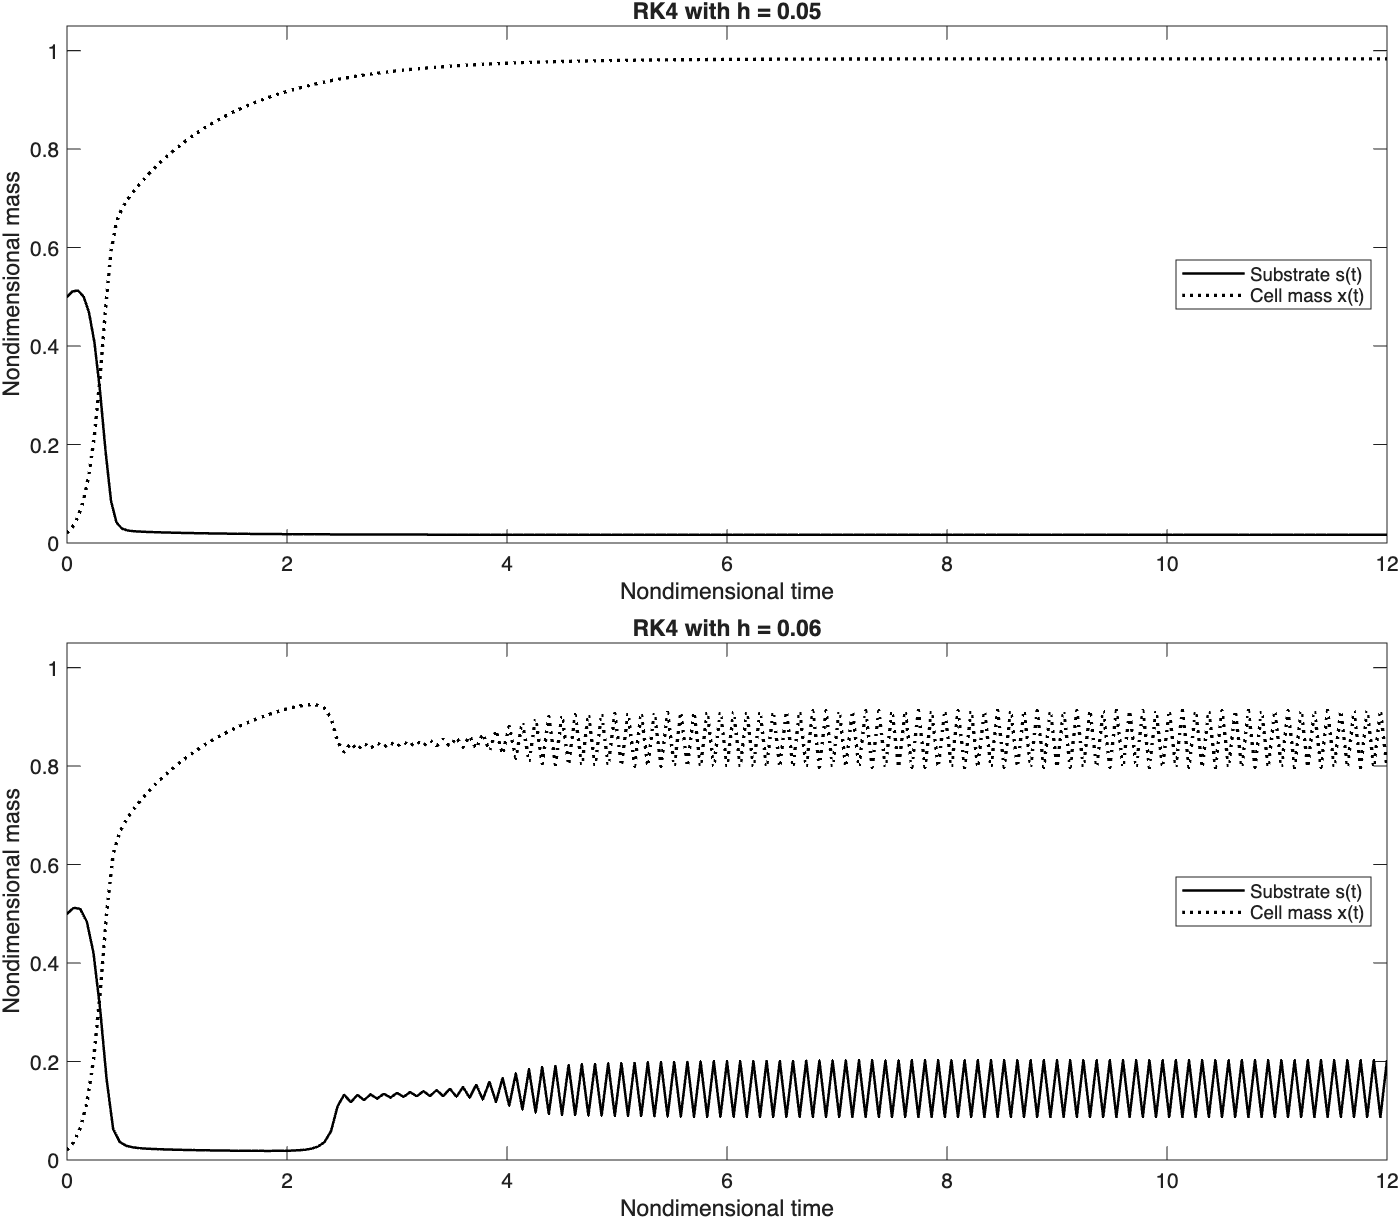
\includegraphics[width=\textwidth]{chemostat_figure.png}
                    \caption{Generated Figure 7.21.}
                    \label{fig:chemostat}
                \end{figure}
            \end{center}
            \begin{center}
                \begin{tabular}{rrrr}\toprule
                    $h$ & Steps & $s_h(12)$ & $x_h(12)$\\\midrule
                    $0.05$ & $240$ & $0.0166667213$ & $0.9833303294$\\
                    $0.06$ & $200$ & $0.2028741247$ & $0.7971229261$\\\bottomrule
                \end{tabular}
            \end{center}
            These plots were generated from the supplied code run in MATLAB R2025b.
            They reproduce the smooth approach to equilibrium and the artificial
            oscillations shown in the supplied textbook figure. The LaTeX source
            embeds the MATLAB data, so no external image or data file is needed
            to compile this document.

            For $h=0.05$, the substrate initially increases slightly because
            $s'(0)=0.286666\ldots>0$, then decreases rapidly as cell mass increases.
            Subsequently the numerical solution approaches
            \[
                (s_*,x_*)=(0.0166666667,0.9833333333),
            \]
            in agreement with the stable-node analysis. The residual difference at
            $t=12$ includes the finite-time transient; an endpoint value need not
            equal its limiting equilibrium exactly.

            \subsection*{3. Why $h=0.06$ gives a different result}
            For the scalar test equation $u'=\lambda u$, one RK4 step multiplies
            the solution by
            \[
                R(z)=1+z+\frac{z^2}{2}+\frac{z^3}{6}+\frac{z^4}{24},\qquad z=h\lambda.
            \]
            A decaying linear mode is numerically damped only if $|R(h\lambda)|<1$.
            On the negative real axis, RK4 is stable for
            $-2.785293563\ldots<z<0$. The fast eigenvalue therefore imposes
            \[
                \boxed{h<\frac{2.785293563\ldots}{55.3125}
                    =0.05035558985\ldots.}
            \]
            The slow eigenvalue $-1$ is stable for both requested steps. For the fast mode,
            \begin{center}
                \begin{tabular}{rrrl}\toprule
                    $h$ & $h\lambda_{\rm fast}$ & $R(h\lambda_{\rm fast})$ & Effect\\\midrule
                    $0.05$ & $-2.765625$ & $0.970748745$ & Perturbations decay\\
                    $0.06$ & $-3.318750$ & $2.150727239$ & Perturbations grow\\\bottomrule
                \end{tabular}
            \end{center}
            Thus $h=0.05$ is just inside the local stability interval, whereas
            $h=0.06$ is outside it. With $h=0.06$, the early transient looks similar,
            but numerical perturbations grow and the trajectory leaves the vicinity
            of the stable equilibrium. The nonlinear RK4 recurrence then develops
            persistent, bounded oscillations, with the substrate too large and the
            cell mass too small. In this run, for $10\le t\le12$,
            \[
                0.0868612\lesssim s_h(t)\lesssim0.2028741.
            \]
            The linear amplification factor is positive, so it predicts growth of
            perturbations, not an alternating linear mode; the subsequent zigzags
            are a property of the nonlinear discrete computation.

            These oscillations are numerical artifacts. In particular, the continuous
            system cannot have a nonconstant periodic orbit: a periodic solution
            would require $s+x=1$ by the total-mass equation, reducing the dynamics
            to a scalar autonomous equation on that line, which has no nonconstant
            periodic solutions. The stable equilibrium has not become unstable in
            the differential equation; the chosen RK4 step has made it unstable
            in the numerical update.

            \subsection*{Verification and MATLAB usage}
            The total mass is an especially useful diagnostic. Because its differential
            equation is linear and the RK4 stages are applied to both components
            together, the discrete solution satisfies, up to rounding,
            \[
                s_n+x_n=1-0.48\,[R(-h)]^n.
            \]
            The script checks this identity to within $10^{-11}$. In the MATLAB run,
            the maximum discrepancy was below $5\times10^{-16}$. Comparison with
            the continuous identity \eqref{eq:mass} gives
            \begin{center}
                \begin{tabular}{rr}\toprule
                    $h$ & $\displaystyle\max_n|s_n+x_n-(1-0.48e^{-t_n})|$\\\midrule
                    $0.05$ & $9.589\times10^{-9}$\\
                    $0.06$ & $2.005\times10^{-8}$\\\bottomrule
                \end{tabular}
            \end{center}
            Even the unstable trajectory has a very accurate total mass. The errors
            in the two components largely cancel, explaining why the artificial
            oscillations in $s$ and $x$ are opposite in phase. Accurate total mass
            alone does not imply accurate individual concentrations.

            Also, numerical stability alone does not imply high accuracy. For
            $h=0.05$, RK4 damps the fast mode by approximately $0.97075$ per step,
            whereas the exact linearized damping is $e^{-2.765625}\approx0.06294$.
            The supplied code includes a finer run with $h=0.005$; the maximum
            difference on the $h=0.05$ grid is approximately $2.273\times10^{-3}$
            for each component. The finer run is an accuracy check, not a substitute
            for either of the two requested plots.
        \end{solution}

        \noindent\textbf{4.} In order to explore absolute stability of RK4, consider the test problem $y'=\lambda y$ with
        $y(0)=1$ and $0\le t\le10$.
        \begin{enumerate}
            \item Analytically apply RK4 to the test problem to show that
            \[
                w_{i+1}=\left(1+h\lambda+\frac12(h\lambda)^2+\frac16(h\lambda)^3+\frac1{24}(h\lambda)^4\right)w_i.
            \]
            This allows us to define $Q(h\lambda)=1+h\lambda+\frac12(h\lambda)^2+\frac16(h\lambda)^3+\frac1{24}(h\lambda)^4$.
            \item Now we will determine the stability region. Allow $h\lambda$ be a complex number
            $h\lambda=x+iy$ where $i=\sqrt{-1}$. Create a contour plot that shows the $|Q|=1$ level
            set over the complex plane. If you are using Matlab, you may find the command
            \texttt{meshgrid} useful for creating a grid of points in the complex plane as follows:
            \begin{lstlisting}[basicstyle=\ttfamily\small,xleftmargin=2.6em]
% Define the grid for the complex plane (z = h*lambda)
x = linspace(-3, 3, 301);
y = linspace(-3, 3, 301);
[X, Y] = meshgrid(x, y);
Z = X + 1i*Y;
            \end{lstlisting}
            \vspace{13pt}
            The Matlab command \texttt{contour()} can then be used to create the requested plot.
            Determine which region in the plot is the stability region.

            \item With $\lambda=-55.31$ determine a bound on $h$ that guarantees $h\lambda$ will lie in the
            stability region for this method. Numerically apply RK4 to the test problem for
            $h$ values inside and outside of this stability region. How do the solution differ?
            How do these results inform the differences you noticed in parts 3(b) and 3(c)?

            \item We will see what happens to numerical solutions with $h\lambda$ combinations that lie in
            both the region of stability and the right half of the complex plane, $\operatorname{Re}(\lambda h)>0$.
            To explore this, set $\lambda=1+20i$ and $h=0.1$. The point $h\lambda$ should now lie in both
            the right half of the plane and in the region of stability -- plot this point and the
            region of stability on the same axes.

            The solution with this $\lambda$ is
            \[
                e^{(1+20i)t}=e^t(\cos(20t)+i\sin(20t)).
            \]
            Should the solution converge to zero as $t\to\infty$? Apply the RK4 to the test
            problem with these values of $\lambda$ and $h$. Does the numerical method converge to
            zero? Should you use a $h\lambda$ that falls in or outside of the stability region for this
            $\lambda$?
        \end{enumerate}

        \begin{solution}
            \leavevmode\par
            \subsection*{(a) Derivation of the amplification polynomial}
            Write $z=h\lambda$ and use the RK4 convention in which each stage
            already contains a factor of $h$. Since $f(t,y)=\lambda y$, the stages are
            \begin{align*}
                k_1&=zw_n,\\
                k_2&=z\left(w_n+\frac{k_1}{2}\right)
                =\left(z+\frac{z^2}{2}\right)w_n,\\
                k_3&=z\left(w_n+\frac{k_2}{2}\right)
                =\left(z+\frac{z^2}{2}+\frac{z^3}{4}\right)w_n,\\
                k_4&=z(w_n+k_3)
                =\left(z+z^2+\frac{z^3}{2}+\frac{z^4}{4}\right)w_n.
            \end{align*}
            Substituting these expressions into the update gives
            \begin{align*}
                w_{n+1}&=w_n+\frac16(k_1+2k_2+2k_3+k_4)\\
                &=\left(1+z+\frac{z^2}{2}+\frac{z^3}{6}+\frac{z^4}{24}\right)w_n.
            \end{align*}
            Thus, for a constant step size and $w_0=1$,
            \[
                \boxed{Q(z)=1+z+\frac{z^2}{2}+\frac{z^3}{6}+\frac{z^4}{24},
                    \qquad w_n=Q(h\lambda)^n.}
            \]
            The exact value is $y(t_n)=e^{\lambda nh}$, so RK4 replaces the exact
            one-step multiplier $e^{h\lambda}$ with its fourth-degree Taylor polynomial.

            \subsection*{(b) Absolute stability region}
            The bounded-amplification region is
            \[
                \boxed{\mathcal S=\{z\in\mathbb C:|Q(z)|\le1\}.}
            \]
            Its interior, where $|Q(z)|<1$, gives $w_n\to0$. On its boundary,
            $|Q(z)|=1$, the magnitude remains constant. Some definitions reserve
            ``absolute stability'' for the strict interior; the plotted boundary
            is the same under either convention.

            The shaded region on the next page is the stable side of the
            $|Q|=1$ contour. It contains $z=-1$, for example, where $Q(-1)=3/8$.
            The exterior gives $|Q|>1$ and amplifies perturbations. The region is
            symmetric about the real axis because $Q$ has real coefficients.
            It is bounded, so classical explicit RK4 is not A-stable.

            \begin{center}
                \begin{figure}
                    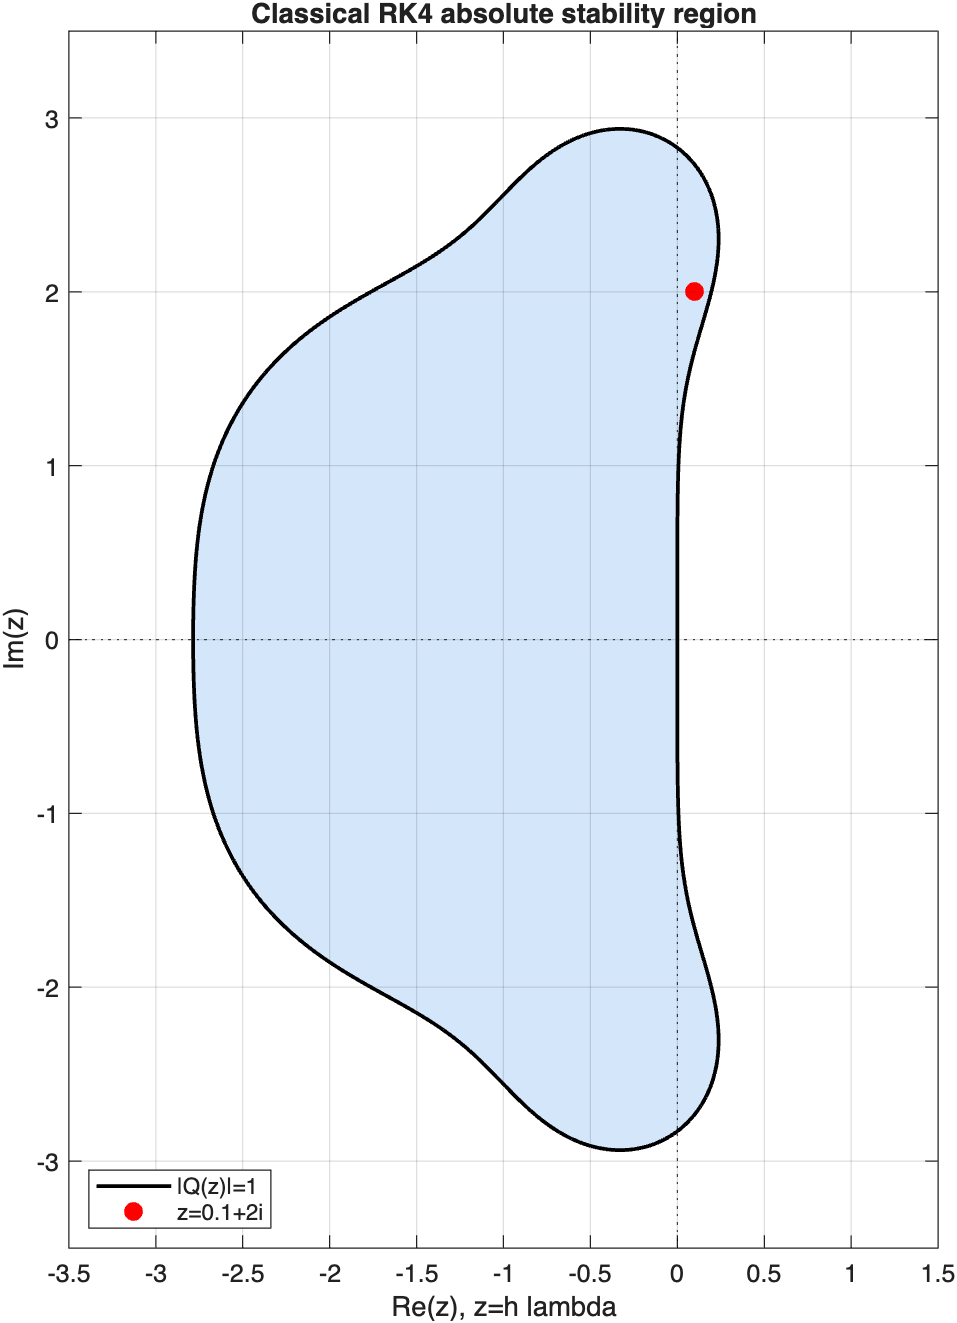
\includegraphics[width=\textwidth]{stability_region.png}
                    \caption{Stability Region.}
                    \label{fig:stabilityregion}
                \end{figure}
            \end{center}
            On the negative real axis, let $z=-r$, $r\ge0$. The nonzero endpoint
            satisfies $Q(-r)=1$, or
            \[
                r^3-4r^2+12r-24=0.
            \]
            Its positive root is $r_*=2.785293563405\ldots$. Thus the real-axis
            interval is $[-r_*,0]$, with strict decay for $-r_*<z<0$.
            On the imaginary axis,
            \[
                |Q(iy)|^2=1+\frac{y^6(y^2-8)}{576},
            \]
            so the imaginary-axis segment runs from $-2\sqrt2\,i$ to $2\sqrt2\,i$.
            The boundary also encloses small areas in the right half-plane;
            part (d) tests one such point.

            \subsection*{(c) The case $\lambda=-55.31$}
            To obtain numerical decay, require $-r_*<-55.31h<0$, hence
            \[
                \boxed{0<h<\frac{2.785293563405\ldots}{55.31}
                    =0.050357865909\ldots.}
            \]
            Equality gives $Q=1$, hence a constant numerical solution rather than
            decay. The two test values are $h=0.05$ (inside) and $h=0.06$ (outside).
            \begin{center}
                \begin{tabular}{rrr}\toprule
                    $h$ & $h\lambda$ & $Q(h\lambda)$\\\midrule
                    $0.05$ & $-2.7655$ & $0.970565404941$\\
                    $0.06$ & $-3.3186$ & $2.150291693782$\\\bottomrule
                \end{tabular}
            \end{center}
            For $h=0.05$, RK4 uses $200$ steps and gives
            \[
                w_{200}=Q(-2.7655)^{200}\approx2.54074706385\times10^{-3}.
            \]
            For $h=0.06$, $10/h$ is not an integer. The script takes $166$ full
            steps to $t=9.96$, followed by one step of length $0.04$. Consequently
            \[
                w(10)=Q(-0.04\cdot55.31)\,Q(-3.3186)^{166}
                \approx6.70479885228\times10^{54}.
            \]
            The last shortened step is included explicitly; it does not undo the
            enormous growth accumulated during the unstable full steps.

            \begin{center}
                \begin{figure}
                    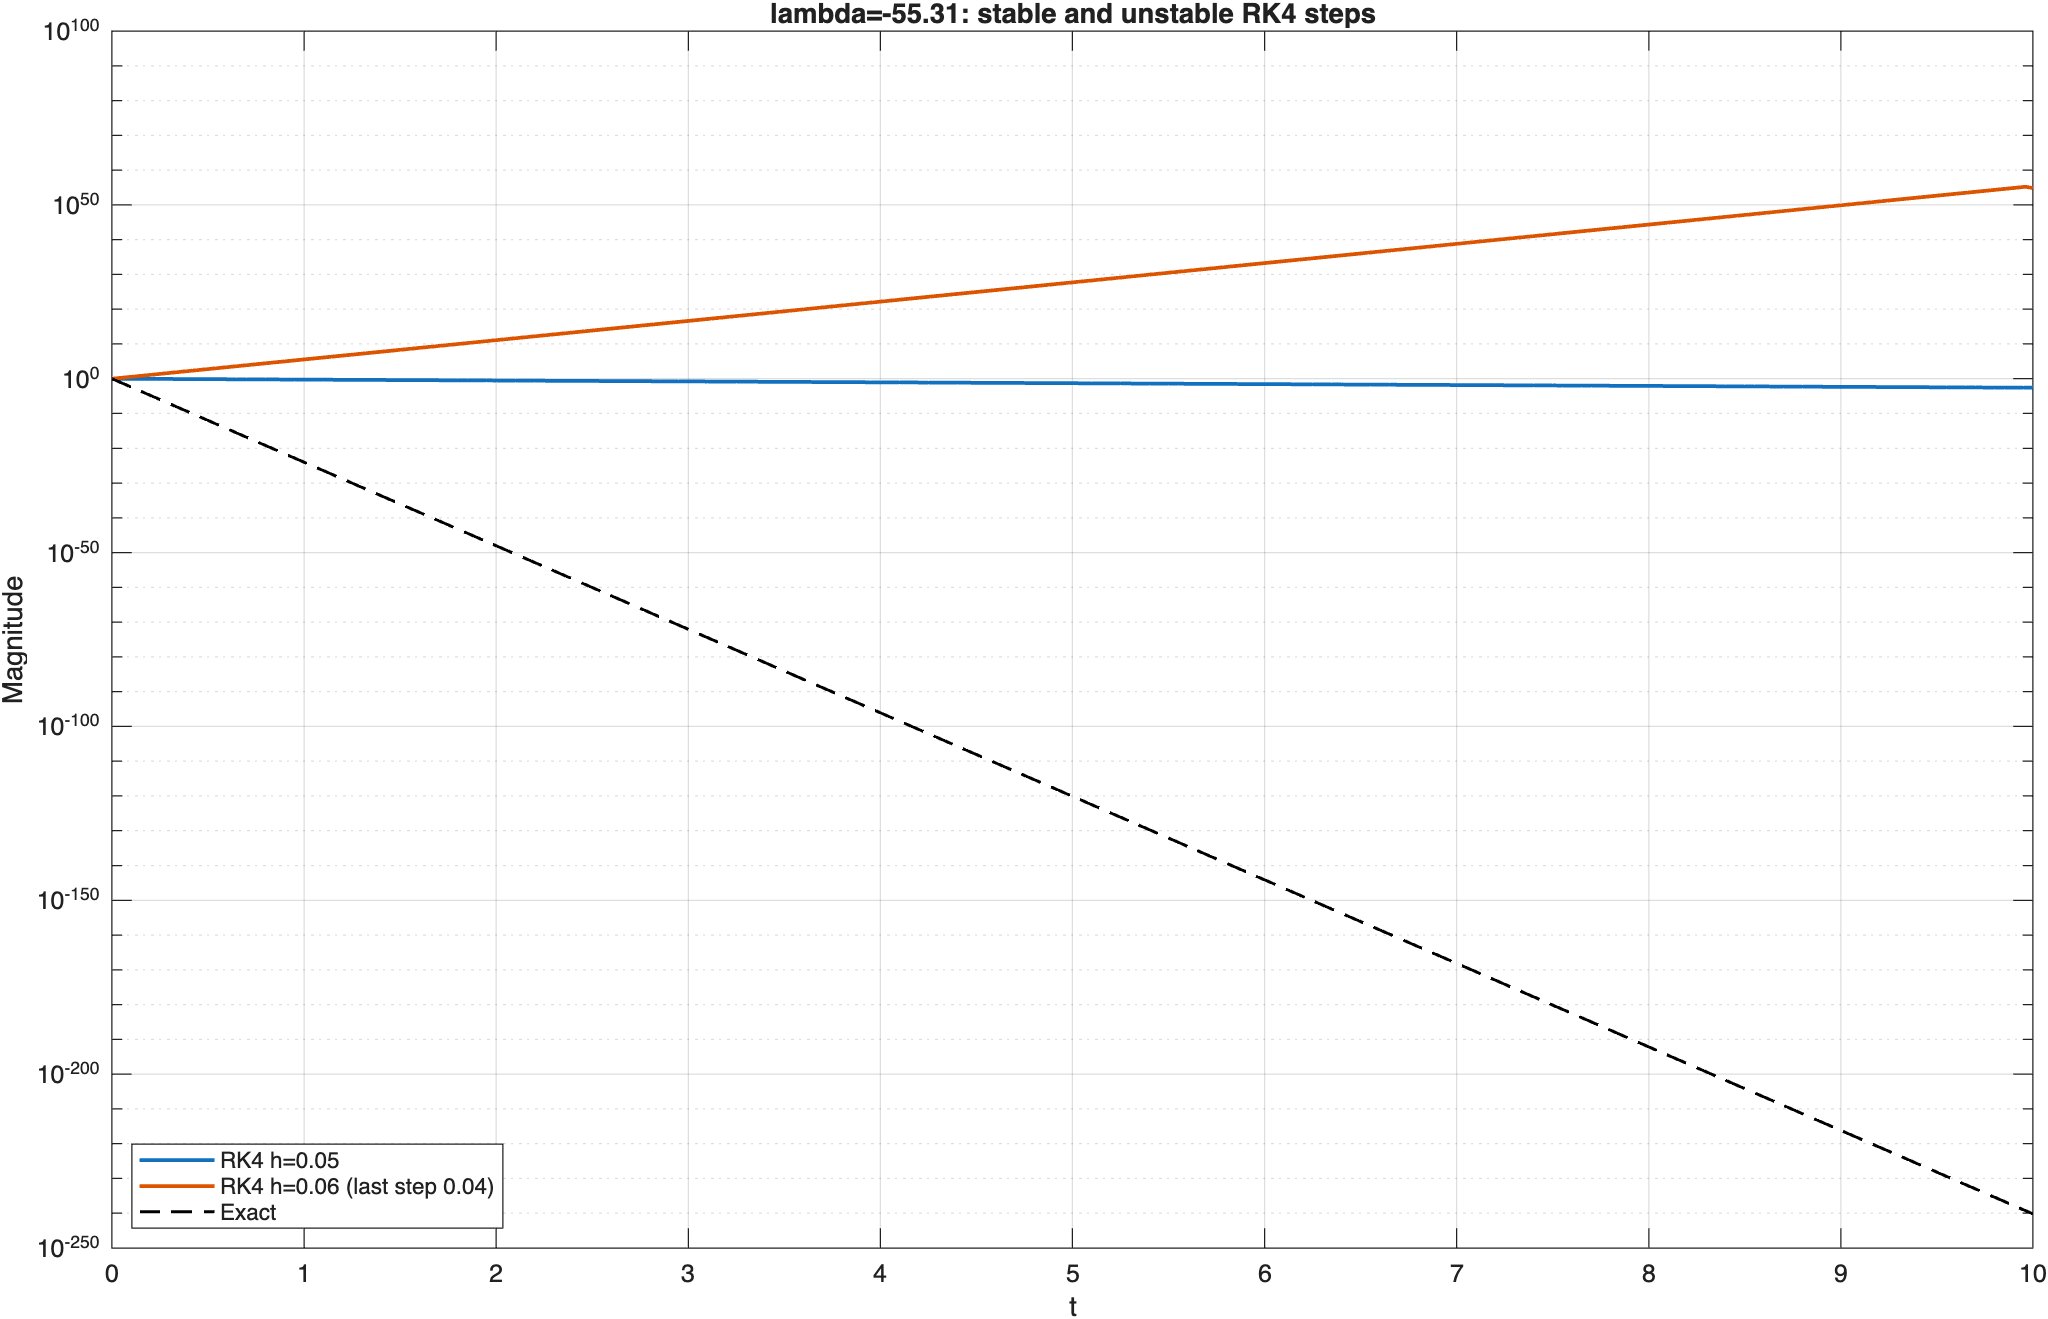
\includegraphics[width=\textwidth]{negative_real_test.png}
                    \caption{Negative Real Test.}
                    \label{fig:negativerealtest}
                \end{figure}
            \end{center}

            The exact solution decays extremely rapidly:
            \[
                y(10)=e^{-553.1}\approx6.19044770713\times10^{-241}.
            \]
            The $h=0.05$ numerical solution also tends to zero as the number of
            steps increases, but much too slowly. This is a clear example of
            \emph{stability without adequate accuracy}. With $h=0.06$, the
            numerical solution grows, although the exact solution decays.

            In Problem 3, the positive chemostat equilibrium has eigenvalues $-1$
            and $-55.3125$. The corresponding fast-mode stability threshold is
            $0.05035558985\ldots$, almost identical to the one here. Thus $h=0.05$
            damps small perturbations of that equilibrium, while $h=0.06$ amplifies
            them. This explains the loss of numerical stability in Problem 3(c).
            The scalar test grows without bound; the chemostat's nonlinear RK4
            recurrence instead develops bounded artificial oscillations. The scalar
            amplification factor diagnoses the initial instability, not the later
            nonlinear waveform.

            \subsection*{(d) The case $\lambda=1+20i$ and $h=0.1$}
            Here $z=h\lambda=0.1+2i$, marked in red on the stability plot.
            Direct evaluation gives
            \[
                Q(0.1+2i)=-0.4381625+0.743666666667i,
                \qquad |Q(0.1+2i)|=0.863149168752<1.
            \]
            Although $\operatorname{Re}(z)>0$, this point is inside the RK4
            stability region. Hence the numerical solution satisfies
            \[
                w_n=Q(0.1+2i)^n,\qquad
                |w_n|=(0.863149168752\ldots)^n\longrightarrow0.
            \]
            In contrast, the exact solution is
            \[
                y(t)=e^{(1+20i)t}=e^t\bigl(\cos(20t)+i\sin(20t)\bigr),
                \qquad |y(t)|=e^t\longrightarrow\infty.
            \]
            Thus the exact solution does \emph{not} converge to zero: it oscillates
            with an exponentially growing amplitude. RK4 with this step size
            produces oscillations with an artificially decaying amplitude.
            At $t=10$ ($n=100$), MATLAB gives
            \[
                \boxed{|w_{100}|\approx4.06055748173\times10^{-7},
                    \qquad |y(10)|=e^{10}\approx2.20264657948\times10^4.}
            \]
            For this growing mode, a useful step must lie \emph{outside} the
            bounded-amplification region so that $|Q(h\lambda)|>1$. However,
            being outside is not sufficient for accuracy: choose $h$ small enough
            that $Q(h\lambda)$ approximates $e^{h\lambda}$ well in both magnitude
            and phase. As $h\to0^+$ along this fixed $\lambda$, this is precisely
            the behavior RK4 recovers. Absolute stability is a condition for
            preserving decay of decaying modes, not a universal prescription
            to damp every differential equation.

            \newpage
            \begin{center}

                \begin{figure}
                    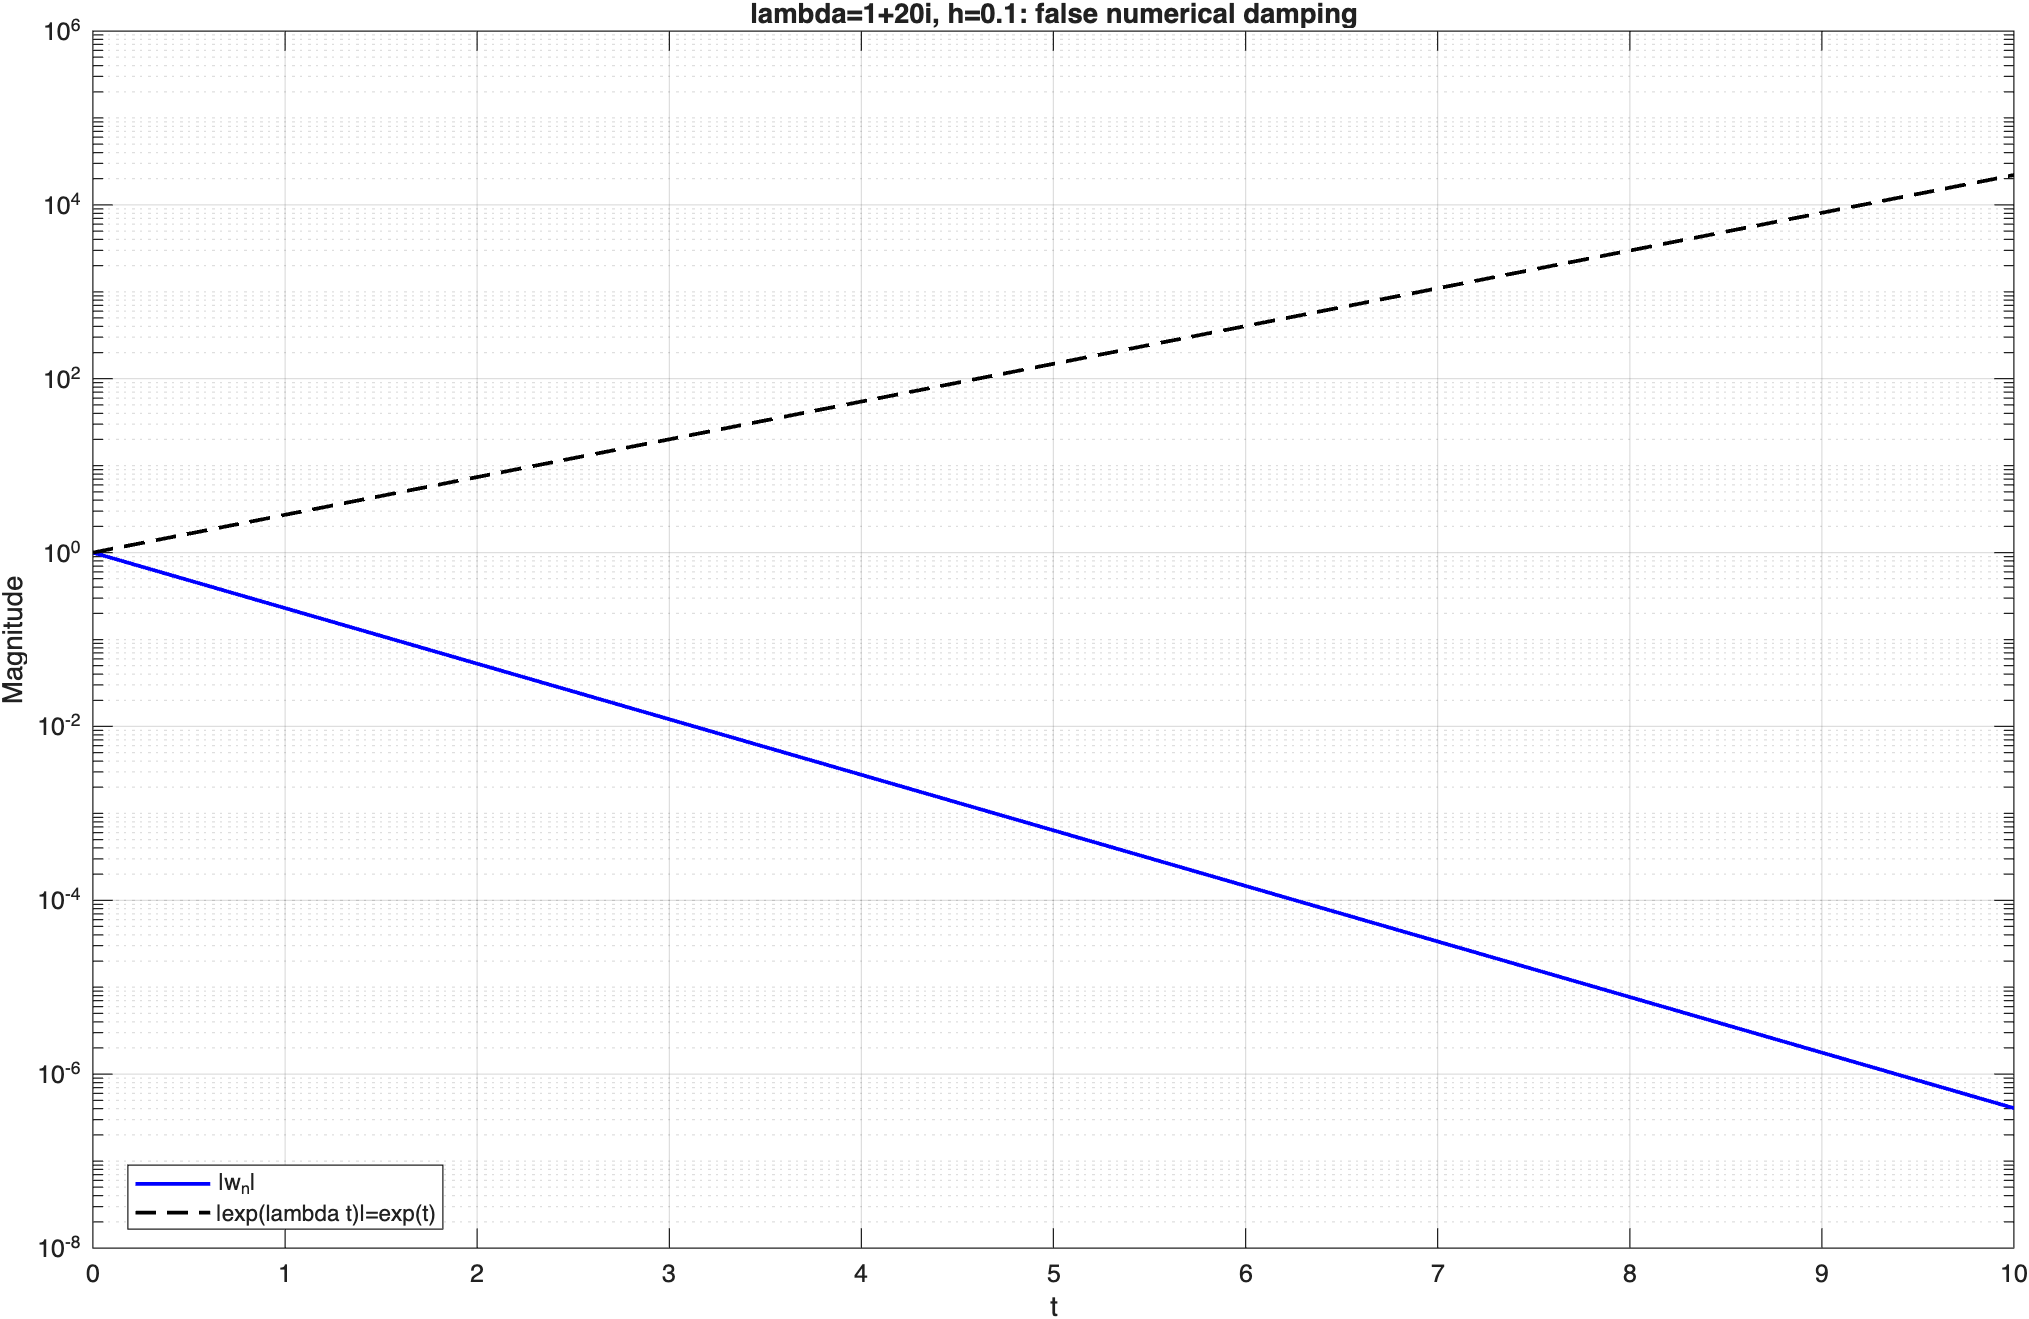
\includegraphics[width=\textwidth]{complex_growth_test.png}
                    \caption{Complex Growth Test.}
                    \label{fig:complexgrowthtest}
                \end{figure}
            \end{center}
        \end{solution}


    \end{onehalfspace}

\end{document}
